\documentclass{article}

% Language setting
% Replace `english' with e.g. `spanish' to change the document language
\usepackage[english]{babel}

% Set page size and margins
% Replace `letterpaper' with`a4paper' for UK/EU standard size
\usepackage[letterpaper,top=2cm,bottom=2cm,left=3cm,right=3cm,marginparwidth=1.75cm]{geometry}

% Useful packages
\usepackage[colorlinks=true, allcolors=blue]{hyperref}
\usepackage{amsmath}
\usepackage{graphicx}
\usepackage{algpseudocode}
\usepackage{algorithm}
\usepackage{amssymb}
\usepackage{xcolor}
\usepackage{tikz}
\usepackage{tikz-qtree}
\usetikzlibrary{automata, positioning, arrows}
\usepackage{amsthm}

\tikzset{
->, % makes the edges directed
>=stealth, % makes the arrow heads bold
node distance=3cm, % specifies the minimum distance between two nodes. Change if necessary.
every state/.style={thick, fill=gray!10}, % sets the properties for each ’state’ node
initial text=$ $, % sets the text that appears on the start arrow
}
\tikzset{
  mydotted/.style={dotted, line width=1pt}
}

\title{\\  \large Theory of Computation \\ \LARGE   Pumping Lemma for CFL}
\author{Mayank Yadav}
\date{April 3, 2025}

\begin{document}
\maketitle


\section{Introduction}
Pumping Lemma for CFL describes an essential characteristic of context-free languages. It says that a string with sufficiently long length belonging to a language that is context-free can be divided into five sections, then the string obtained by pumping(or repeating) the second and third sections also belongs to the same language.

\begin{center}
\fbox{%
    \parbox{0.9\textwidth}{
        Pumping Lemma for context-free languages states that for a given context-free language $L$, there exists an integer $p\ge 1$ such that for every string $s$ having $\mid s \mid \ge p$ can be expressed as $s=uvwxy$ and the following conditions hold:\\
        $$\mid vx\mid \ge 1$$ 
        $$\mid vwx\mid \le p$$
        $$(\forall n\ge 0) (uv^nwx^ny\in L) $$
        Mathematically,
        $$
        \forall L \subseteq \Sigma^*, \text{context-free}(L) 
        $$
        $$
        \implies  \exists p \geq 1, \forall s \in L, \mid s\mid  \geq p 
        $$
        $$
        \implies  \exists u, v, w, x, y \in \Sigma^*, (s = uvwxy) \land (\mid vx\mid  \geq 1) \land (\mid vwx\mid  \leq p) \land (\forall n \geq 0, uv^nwx^ny \in L)
        $$
    }
}
\end{center}

We can get intuitions behind this lemma by considering a parse tree of a sufficiently long string $s$ that belongs to context-free language $L$ and let $G$ be the context-free grammar that generates $L$. As $s\in L$, it can be derived from grammar $G$. As the string $s$ is of sufficiently long length($\mid s\mid \ge p$),and the number of non-terminal symbols in the grammar is finite, there must be some non-terminal symbol $R$ that appears more than once according to pigeonhole principle. 

We can repeat this $R$ to pump the string and as a result pump $v$ and $x$ in the string $s$ to obtain $s'=uv^iwx^iy$ where $i\ge 0$ which also belongs to the same language $L$.

\begin{figure}
  \centering 
    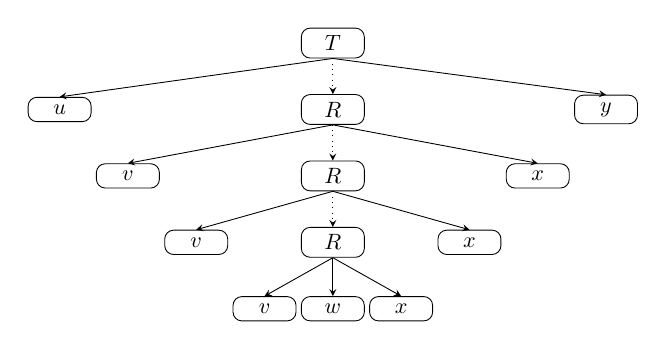
\begin{tikzpicture}[scale=0.8,every tree node/.style={draw, rounded corners, align=center, minimum width=1cm}]
      \Tree [.{$T$} 
              {$u$} 
              \edge[dotted]; [.{$R$} 
                          {$v$} 
                          \edge[dotted]; [.{$R$} 
                                      {$v$} 
                                      \edge[dotted]; [.{$R$} 
                                                  {$v$} 
                                                  {$w$} 
                                                  {$x$} 
                                              ]
                                      {$x$} 
                                  ]
                          {$x$} 
                      ]
              {$y$} 
      ]
  \end{tikzpicture}
\caption{Illustration of the pumping lemma using a parse tree}
\label{fig:my_label}
\end{figure}

\section{Application:}
Pumping lemma can be used to prove that a language is non context-free by "Proof by Contradiction". We assume that the language is context-free and choose a string whose length is greater than the pumping constant and that can't be pumped and we reach a contradiction by failing to divide the string into any $u,v,w,x,y$ and then put forward that the language is non context-free.

It is important to note that the converse of pumping lemma is not true i.e. a language that satisfies these conditions is not necessarily a context-free language.

\subsection{Example 1}

Prove that the language $L=\{a^nb^nc^n\mid n\ge 0\}$ is not context-free.

\begin{proof}
Let us assume $L$ to be a CFL. Now according to pumping lemma $\exists(p\ge1)$.
Let the string $s\in L$ and $$s=a^pb^pc^p$$ $$\mid s\mid=3p>p $$ $$s=uvwxy$$
Two cases arise:

\textbf{Case 1:} $v$ and $x$ each contains only one type of symbol.
Now by statement 3 of lemma, $s'=uv^2wx^2y\in L$ but $s'$ doesn't contain equal number of $a$'s, $b$'s and $c$'s so $s'\notin L$. A contradiction.

\textbf{Case 2:} $v$ and $x$ each contains two types of symbols.
Now by statement 3 of lemma, $s'=uv^2wx^2y\in L$ but in $s'$ the symbols are not in correct order and are intermixed so $s'\notin L$. A contradiction.

Hence, the initial assumption was wrong and the language $L$ is not context-free.
\end{proof}

\subsection{Example 2}

Prove that the language $L=\{a^ib^jc^k\mid 0\le i\le j \le k\}$ is not context-free.

\begin{proof}
Let us assume $L$ to be a CFL. Now according to pumping lemma $\exists(p\ge1)$.
Let the string $s\in L$ and $$s=a^pb^pc^p$$ $$\mid s\mid=3p>p $$ $$s=uvwxy$$
Two cases arise:

\textbf{Case 1:} $v$ and $x$ each contains only one type of symbol.
Now 3 further cases arise:
\begin{itemize}
    \item \textbf{Case 1a } $a$'s don't appear: In this case, pumping up won't help as number of $b$'s and $c$'s can be more than the number of $a$'s. So we have to pump down to reach a contradiction. By statement 3 of lemma $s'=uv^0wx^0y \in L$ but it contains same number of $a$'s as $s$ but lesser $b$'s and $c$'s so $s'\notin L$. A contradiction. 
    
    \item \textbf{Case 1b } $b$'s don't appear: $v$ and $x$ contains $a$'s or $c$'s. For $a$'s,if we pump up the $s$ then by statement 3 of lemma $s_1'=uv^2wx^2y \in L$ but it contains more number of $a$'s than $b$'s so $s_1'\notin L$. A contradiction.  For $c$'s, if we pump down the $s$ then by statement 3 of lemma $s_2'=uv^0wx^0y \in L$ but it contains less number of $c$'s than $b$'s so $s_2'\notin L$. A contradiction.
    
    \item \textbf{Case 1c } $c$'s don't appear: By statement 3 of lemma $s'=uv^2wx^2y \in L$ but it contains more number of $a$'s or $b$'s than $c$'s so $s'\notin L$. A contradiction. 
    
\end{itemize}

\textbf{Case 2:} $v$ and $x$ each contains two types of symbols.
Now by statement 3 of lemma, $s'=uv^2wx^2y\in L$ but in $s'$ the symbols are not in correct order and are intermixed so $s'\notin L$. A contradiction.

Hence, the initial assumption was wrong and the language $L$ is not context-free.
\end{proof}

\subsection{Example 3}

Prove that the language $L=\{ww\mid w \in \{0,1\}^*  \}$ is not context-free.

\begin{proof}
Let us assume $L$ to be a CFL. Now according to pumping lemma $\exists(p\ge1)$.
Let the string $s\in L$ and $$s=0^p1^p0^p1^p$$ $$\mid s\mid=4p>p $$ $$s=uvwxy$$
By condition 2 of the pumping lemma, $|vwx| \leq p$. 

3 cases arise:

\textbf{Case 1} We chose $vwx$ in the first half of $s$: By statement 3 of lemma, $s'=uv^2wx^2y\in L$ but now the first symbol of second half becomes $1$ but the first symbol of first half is still $0$. So $s'\notin L$. A contradiction.

\textbf{Case 2} We chose $vwx$ in the second half of $s$: By statement 3 of lemma, $s'=uv^2wx^2y\in L$ but now the last symbol of first half becomes $0$ but the last symbol of second half is still $1$. So $s'\notin L$. A contradiction.

\textbf{Case 3} We chose $vwx$ ranging over both first half and second half of $s$: By statement 3 of lemma, $s'=uv^0wx^0y\in L$ but $s'=0^p1^i0^j1^p$ where  $(i< p \vee j < p)$ so $s'\notin L$. A contradiction.

Hence, the initial assumption was wrong and the language $L$ is not context-free.
\end{proof}

\subsection{Example 4}

Prove that the language $L=\{0^{n}\#0^{2n}\#0^{3n} \mid n\ge0  \}$ is not context-free.

\begin{proof}
Let us assume $L$ to be a CFL. Now according to pumping lemma $\exists(p\ge1)$.
Let the string $s\in L$ and $$s=0^{p}\#0^{2p}\#0^{3p}$$ $$\mid s\mid=6p+2>p $$ $$s=uvwxy$$
By condition 2 of the pumping lemma, $|vwx| \leq p$. 

2 cases arise:

\textbf{Case 1:} $v$ contains \# or $x$ contains \# .
Now by statement 3 of lemma, $s'=uv^2wx^2y\in L$ but $s'$ contains more than two \#s so $s'\notin L$. A contradiction.

\textbf{Case 2:} $v$ doesn't contains \# and $x$ doesn't contains \# . So $vwx$ ranges over segments $0^{p}$ or $0^{2p}$ or $0^{3p}$.
Now by statement 3 of lemma, $s'=uv^2wx^2y\in L$ but in $s'$ the $0$'s are not in ratio $1:2:3$ so $s'\notin L$. A contradiction.

Hence, the initial assumption was wrong and the language $L$ is not context-free.
\end{proof}

\subsection{Example 5}

Prove that the language $L=\{ w\#t \mid w \text{ is a substring of } t \text{ where } w, t \in \{a, b\}^* \}$ is not context-free.

\begin{proof}
Let us assume $L$ to be a CFL. Now according to pumping lemma $\exists(p\ge1)$.
Let the string $s\in L$ and $$s=a^pb^p\#a^pb^p$$ $$\mid s\mid=4p+1>p $$ $$s=uvwxy$$
By condition 2 of the pumping lemma, $|vwx| \leq p$. 

4 cases arise:

\textbf{Case 1:} $v$ contains \# or $x$ contains \# .
Now by statement 3 of lemma, $s'=uv^2wx^2y\in L$ but $s'$ contains more than one \#s so $s'\notin L$. A contradiction.

\textbf{Case 2:}  $vwx$ lies on left of $\#$. By statement 3 of lemma, $s'=uv^2wx^2y\in L$ but in $s'$ the left of $\#$ is longer and hence it can't be a substring so $s'\notin L$. A contradiction.

\textbf{Case 3:}  $vwx$ lies on right of $\#$. By statement 3 of lemma, $s'=uv^0wx^0y\in L$ but in $s'$ the left of $\#$ is longer and hence it can't be a substring so $s'\notin L$. A contradiction.

\textbf{Case 4:} $v$ doesn't contains \# and $x$ doesn't contains \# and $vwx=b^i\#a^j$ where $i<p\wedge j<p\wedge (i+j\ge p-1)$. Now by statement 3 of lemma, $s'=uv^2wx^2y\in L$ but in $s'$ the left of $\#$ contains more number of $b$'s and hence it can't be a substring so $s'\notin L$. A contradiction.

Hence, the initial assumption was wrong and the language $L$ is not context-free.
\end{proof}

\subsection{Example 6}

Prove that the language $L=\{ 0^n1^n0^n1^n \mid n\ge 0\}$ is not context-free.

\begin{proof}
Let us assume $L$ to be a CFL. Now according to pumping lemma $\exists(p\ge1)$.
Let the string $s\in L$ and $$s=0^p1^p0^p1^p$$ $$\mid s\mid=4p>p $$ $$s=uvwxy$$
By condition 2 of the pumping lemma, $|vwx| \leq p$.

2 cases arise:

\textbf{Case 1:} $v$ and $x$ each contains only one type of symbol.
Now by statement 3 of lemma, $s'=uv^2wx^2y\in L$ but $s'$ doesn't contain equal number of $0$'s and $1$'s in ratio $1:1:1:1$ so $s'\notin L$. A contradiction.

\textbf{Case 2:} $v$ and $x$ each contains two types of symbols.
Now by statement 3 of lemma, $s'=uv^2wx^2y\in L$ but in $s'$ the symbols are not in correct order and are intermixed so $s'\notin L$. A contradiction.


Hence, the initial assumption was wrong and the language $L$ is not context-free.
\end{proof}

\begin{thebibliography}{9}
\bibitem{sipser}

Michael Sipser,
\textit{Introduction to the Theory of Computation},
Cengage Learning, 2012.

\bibitem{enwiki:1264121825}
Wikipedia contributors,
\textit{Pumping lemma for context-free languages --- Wikipedia, The Free Encyclopedia},
2025,
\url{https://en.wikipedia.org/wiki/Pumping_lemma_for_context-free_languages},


\end{thebibliography}

\end{document}

